\documentclass[12pt,a4paper]{article}


\setlength{\textwidth}{165mm}
\setlength{\textheight}{240mm}
\setlength{\parindent}{0mm} % S{\aa} meget rykkes ind efter afsnit
\setlength{\parskip}{\parsep}
\setlength{\headheight}{0mm}
\setlength{\headsep}{0mm}
\setlength{\hoffset}{-2.5mm}
\setlength{\voffset}{0mm}
\setlength{\footskip}{15mm}
\setlength{\oddsidemargin}{0mm}
\setlength{\topmargin}{0mm}
\setlength{\evensidemargin}{0mm}

%til tables!
\usepackage[T1]{fontenc}
\usepackage[utf8]{inputenc}
% jubiii
\usepackage{tabularx,ragged2e,booktabs,caption}
\usepackage{algorithm,algpseudocode}
\usepackage[T1]{fontenc}
\usepackage[all]{xy}
\usepackage{graphicx}    % For grafik (billederfiler)
\usepackage[T1]{fontenc} % For at blande \textsc{} med \textbf{}
\usepackage[utf8]{inputenc}
\usepackage{amsfonts,amsmath,amssymb}
\usepackage{eucal}
\usepackage[danish]{babel}
\usepackage{enumerate}  
\usepackage{hyperref}
\usepackage{url}
\usepackage{array}
\usepackage{mathptmx}
\usepackage{amsmath}
\usepackage{multirow}
\usepackage[dvipsnames,usenames]{color}
\usepackage{tabularx,colortbl,xcolor}

\setlength{\textwidth}{165mm}
\setlength{\textheight}{240mm}
\setlength{\parindent}{0mm} % S{\aa} meget rykkes ind efter afsnit
\setlength{\parskip}{\parsep}
\setlength{\headheight}{0mm}
\setlength{\headsep}{0mm}
\setlength{\hoffset}{-2.5mm}
\setlength{\voffset}{0mm}
\setlength{\footskip}{15mm}
\setlength{\oddsidemargin}{0mm}
\setlength{\topmargin}{0mm}
\setlength{\evensidemargin}{0mm}

%til tables!
\usepackage[T1]{fontenc}
\usepackage[utf8]{inputenc}
% jubiii
\usepackage{tabularx,ragged2e,booktabs,caption}
\usepackage{float}
\usepackage[T1]{fontenc}
\usepackage[all]{xy}
\usepackage{graphicx}    % For grafik (billederfiler)
\usepackage[T1]{fontenc} % For at blande \textsc{} med \textbf{}
\usepackage[utf8]{inputenc}
\usepackage{amsfonts,amsmath,amssymb}
\usepackage{eucal}
\usepackage[danish]{babel}
\usepackage{enumerate}  
\usepackage{hyperref}
\usepackage{url}
\usepackage{array}
\usepackage{mathptmx}
\usepackage{amsmath}
\usepackage{multirow}
\usepackage[dvipsnames,usenames]{color}
\usepackage{tabularx,colortbl,xcolor}
\hypersetup{%
    pdfborder = {0 0 0}
}

\DeclareSymbolFont{usualmathcal}{OMS}{cmsy}{m}{n}
\DeclareSymbolFontAlphabet{\mathcal}{usualmathcal}

% til tables
\newcolumntype{C}[1]{>{\Centering}m{#1}}
\renewcommand\tabularxcolumn[1]{C{#1}}
% jubiii


\begin{document}
\title{Organic Donkey Hostel - Hjemmeside med booking\\
Projektkursus Systemudvikling 2015}
\maketitle
\begin{center}
Projektgruppe-nummer 1, gruppemedlemmer:
\end{center}
\begin{center}
Jeppe Schönemann Skov 240992\\
Rose Sofie Greve 250493\\
Frederik Leed Henriksen 110394\\
\end{center}
\begin{center}
Instruktor: Christoffer Wadum\\ \hfill \\ \hfill \\ 
\end{center}
\newpage
\tableofcontents
\newpage
\section{Abstract}
We are making a website for a small Bed and Breakfast on Isla Margarita, Venezuela. The place is working towards becoming a sustainable and self-sufficient mini-hostel, where guests can enjoy organic greens from the garden.
The frontpage on the website will contain a description of the place and the surrounding area.
The website will contain a simple booking- and online payment system.
The website will have a link with pictures of the houses and surrounding facilities, and a link with information on the different activities taking place at the hostel.
With courtesy to the place working with ecology and sustainability, the layout of the website will be simple and inspired by the colors of nature.
Further, we will make an administration part of the system, from where our costumer can see and edit the bookings. The administrator will also be able to edit the website photos and text descriptions. \\\\
\newpage
\section{IT-projektets formål og rammer}
Her følger en beskrivelse af rammerne for vores IT-projekt, baseret på FACTOR-begrebet.
\\\\
Functionality: Skal indeholde et booking- og betalingssystem, hvor administratoren har mulighed for at redigere i bookingerne. Samt redigere i de billeder og den information der fremvises på hjemmesiden. \\

Application domain: Skal administrere bookninger, herunder redigere og slette bookinger samt finde kontaktoplysninger på de personer der har oprettet en booking.\\
 
Conditions:  Vi skal udvikle et simpelt system, da de der skal betjene systemet har ikke stor teknisk erfaring.\\

Technology: Systemet skal både udvikles og kunne betjenes på en billig pc med internet. Grundet hyppige strømsvigt skal databasen ligge på en webserver. \\

Objects: Personer der ønsker at booke værelse. Administrering af bookinger og websiden.\\

Responsibility: Systemet skal løse administrative problematikker i henhold til at holde styr på kontaktoplysninger af kunder, holde styr på hvilke værelser der er ledige, og hvornår disse er ledige. Systemet skal også reklamere for hostel'et.\\
\newpage
\section{Kravspecifikationer for IT-løsningen}
\subsection{a - Funktionelle og ikke funktionelle krav}
Dette afsnit angiver de funktionelle og ikke funktionelle krav, samt de begrænsninger vi har til vores system.\\\\
\textbf{Funktionelle krav:} \\
- Side med bookingsystem der giver brugeren mulighed for at booke senge\\
- Administrativ side der giver vores kunde mulighed for at redigere i bookinger, tekst og billeder på brugersiden\\
- Loginsystem til den administrative side\\
- Betalingssystem. Et eksternt system som kunden viderestilles til. Ikke et betalingssystem vi selv koder.\\\\
       \textbf{Ikke-funktionelle krav:} \\
- Simpelt system som kan benyttes af folk uden særlig teknisk erfaring\\
- Side med information om stedet\\
- Side med billedegalleri\\
- Side med kontaktinformation\\
- Layout der afspejler hostelets stil og holdning til miljøet. \\\\
      \textbf{Begrænsninger:} \\
	Siden skal kunne vises på en billig computer og uden hurtigt internet til rådighed. Databasen med bookinger skal ligge på en webserver, da strømsvigt er hyppige i området.
\newpage
\subsection{b - Use case model}
Dette afsnit beskriver kort det mest essentielle ved systemets use cases, og illustrerer sammenhængen mellem disse og aktørerne i et højniveau-diagram. 
\begin{figure}[H]
\centering
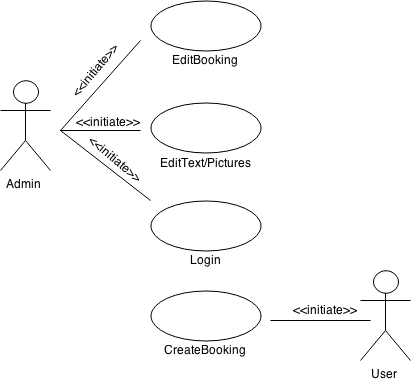
\includegraphics[scale=0.7]{hoejniveau.png}
\caption{Et højniveau-diagram der illustrerer hvilke use cases de forskellige aktører har}
\end{figure}
\textbf{EditBooking}  Administratoren kan slette og redigere i værelsesbookingerne. Login er krævet for at kunne redigere i bookinger.\\
\textbf{EditText/Pictures} Administratoren kan slette og redigere i teksten og billederne på hjemmesiden. Login er krævet for at kunne redigere i hjemmesiden.\\
\textbf{Login} Administartoren skal logge ind på Admin siden, for at se og redigere bookinger samt tekst og billeder.\\
\textbf{CreateBooking} Brugeren kan booke et værelse på hostelet gennem hjemmesiden.\\
\newpage
\subsection{c - Use cases}
De følgende tre tabeller angiver mere detaljerede beskrivelser at vores tre vigtigeste use cases. Diagrammerne illusterer relationerne mellem aktørerne og systemet. \\\\
\begin{minipage}{\textwidth}

\captionof{table}{Højniveau use-case-diagram over use casen Login} \label{tab:title}
\begin{tabular}{| p{5cm} p{10cm} |}
\hline Use-case-name & Login \\
\hline Participating actors & Administratoren \\
\hline Flow of events & \begin{enumerate}
\item Administratoren indtaster sit brugernavn og kodeord på admin log-in siden og trykker på log-in knappen
\item Admin-databasen bliver spurgt om de indsendte oplysninger er rigtige.
\item Hvis der findes et match, bliver man videreført til admin-siden. Hvis ikke får man en fejlmeddelelse.
\end{enumerate} \\
\hline Entry conditions & At man ikke allerede er logget ind \\
\hline Exit conditions & At man er logget ind \\
\hline
\end{tabular}

\end{minipage}

\bigskip

\begin{minipage}{\textwidth}

\captionof{table}{Højniveau use-case-diagram over use casen EditBooking} \label{tab:title}
\begin{tabular}{| p{5cm} p{10cm} |}
\hline Use-case-name & EditBooking \\
\hline Participating actors & Administratoren \\
\hline Flow of events & \begin{enumerate}
\item Administratoren indtaster den ønskede ændring for en booking
\item Ændringen bliver sendt til databasen og bookingens detaljer redigeres
\item Tabellen opdateres med de nye oplysninger
\end{enumerate} \\
\hline Entry conditions & At man er logget ind \\
\hline Exit conditions & At den ønskede ændring i bookingen er sket \\
\hline
\end{tabular}

\end{minipage}
	
\bigskip

\begin{minipage}{\textwidth}

\captionof{table}{Højniveau use-case-diagram over use casen CreateBooking} \label{tab:title}
\begin{tabular}{| p{5cm} p{10cm} |}
\hline Use-case-name & CreateBooking \\
\hline Participating actors & Brugeren \\
\hline Flow of events & \begin{enumerate}
\item Kunden indtaster sine ønskede booking datoer og kontaktinformationer 
\item Kunden trykker på booking-knappen og bookinginformationerne bliver tjekket for at verificere at bookingen ikke overlapper med andre bookinger
\item Hvis datoerne for bookingen godkendes, bliver bookingen oprettet, og kunden bliver videresendt til "home" siden. Hvis der er overlap får kunden en fejlmeddelelse.
\end{enumerate} \\
\hline Entry conditions & At brugeren befinder sig på bookingsiden \\
\hline Exit conditions & At brugerens booking gemmes i databasen  \\
\hline
\end{tabular}

\end{minipage}	
	
\subsection{d - Klassediagram over problemområdet}
Dette afsnit illustrerer vores problemområder i et klassediagram.\\
Figur 2 illustrerer et klassediagram over problemområdet  bookingsystem. Application() tilføjer, redigerer og sletter bookinger fra bookingdatabasen. Booking definerer hvilke parametre en booking skal indeholde.
\begin{figure}[H]
\centering
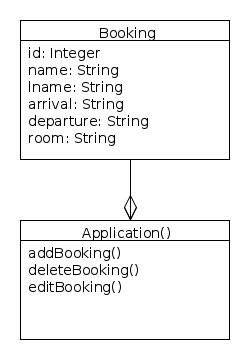
\includegraphics[scale=0.6]{BookingSystem.jpg}
\caption{UML klassediagram over bookingsystemet}
\end{figure}
\subsection{e - BCE-model}
Dette afsnit indeholder en BCE-model over vores system.\\\\
\begin{minipage}{\textwidth}

\captionof{table}{Boundary} \label{tab:title}
\begin{tabular}{| p{5cm} | p{10cm} |}
\hline Admin log-in side & Web-siden for administratoren som benyttes til at verificere at personen er administrator \\
\hline Kunde booking web-side & Her har kunden adgang til at oprette en booking samt navigering til de andre kunde sider \\
\hline Kunde "home" web-side & Her kan kunden navigere til de andre sider \\
\hline Kunde galleri web-side & Her kan kunden navigere til de andre sider \\
\hline Kunde kontakt web-side & Her kan kunden navigere til de andre sider \\
\hline Kunde aktiviteter web-side & Her kan kunden navigere til de andre sider \\
\hline
\end{tabular}

\end{minipage}

\bigskip

\begin{minipage}{\textwidth}

\captionof{table}{Control} \label{tab:title}
\begin{tabular}{| p{5cm} | p{10cm} |}
\hline Admin log-in \newline verificeringsknappen & Facilliterer forespørgelsen mellem admin log-in siden og admin-databasen. Hvis personen er en admin, bliver vedkommende sendt videre til admin siden. Hvis ikke, sker der ikke noget\\
\hline Opret booking knap & Søger databasen for overlap i dato. Hvis der ikke er sådanne konflikter skabes en booking med de givne informationer i databasen. Hvis der er en konflikt vises en passende fejlmeddelelse \\
\hline Rediger booking knap & Redigerer i en allerede oprettet booking i databasen \\
\hline Rediger web-sider & Redigerer kundesidernes indhold i forhold til billeder og tekst (Vi ved endnu ikke hvordan dette skal implementeres) \\
\hline "Home" link & Sender kunden til "home" web-page \\
\hline Booking link & Sender kunden til booking web-page \\
\hline Galleri link & Sender kunden til galleri web-page \\
\hline Kontakt link & Sender kunden til kontakt web-page \\
\hline Aktiviteter link & Sender kunden til aktiviteter web-page \\
\hline
\end{tabular}

\end{minipage}

\bigskip

\begin{minipage}{\textwidth}

\captionof{table}{Entity} \label{tab:title}
\begin{tabular}{| p{5cm} | p{10cm} |}
\hline Admin databasen & Indeholder oplysninger om hvilke brugere der eksisterer i systemet \\
\hline Administrator siden & Her har administrator mulighed for at tilse aktuelle bookninger og rette i databasen \\
\hline Booking database & Indeholder alle bookinger på siden \\
\hline
\end{tabular}

\end{minipage}
\newpage
\subsection{f - Sekvensdiagrammer over use cases}
De følgende sekvensdiagrammer illusterer interaktionen mellem aktøren og systemet i en use case.\\ 
\begin{figure}[H]
\centering
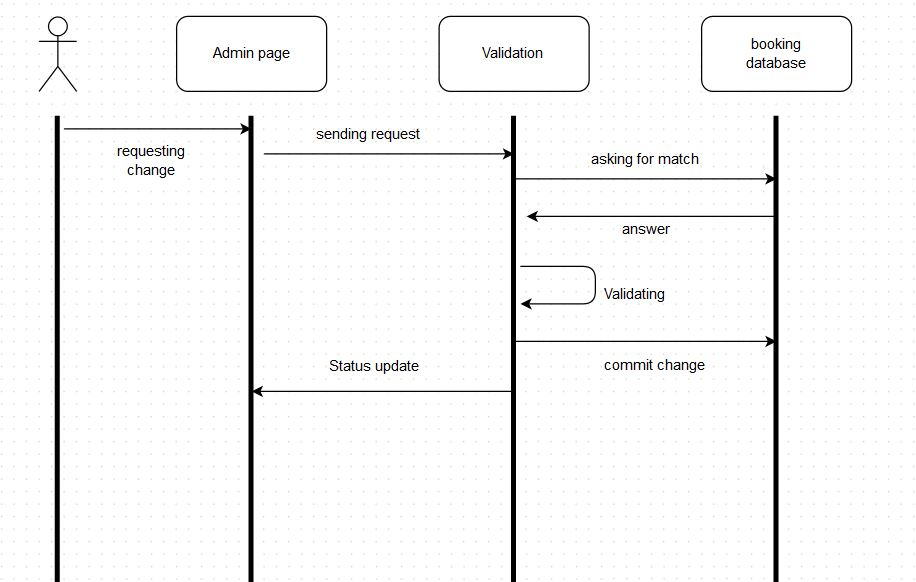
\includegraphics[scale=0.6]{adminInteraction.jpg}
\caption{Sekvens-diagram over use-casen EditBooking}
\end{figure}
Figur 3: Brugeren forespørger om en ændring fra admin siden. 
Fra admin siden sendes en forespørgsel til en funktion, der validerer denne. 
Funktionen sender en forespørgsel til databasen, som svarer.
Hvis valideringsfunktionen evaluerer til "sand", 
bliver ændringen i databasen gennemført.
Hvis ikke bliver det skridt sprunget over.
Man får en statusopdatering, der beskriver, om ændringen bliver udført eller ej.
\begin{figure}[H]
\centering
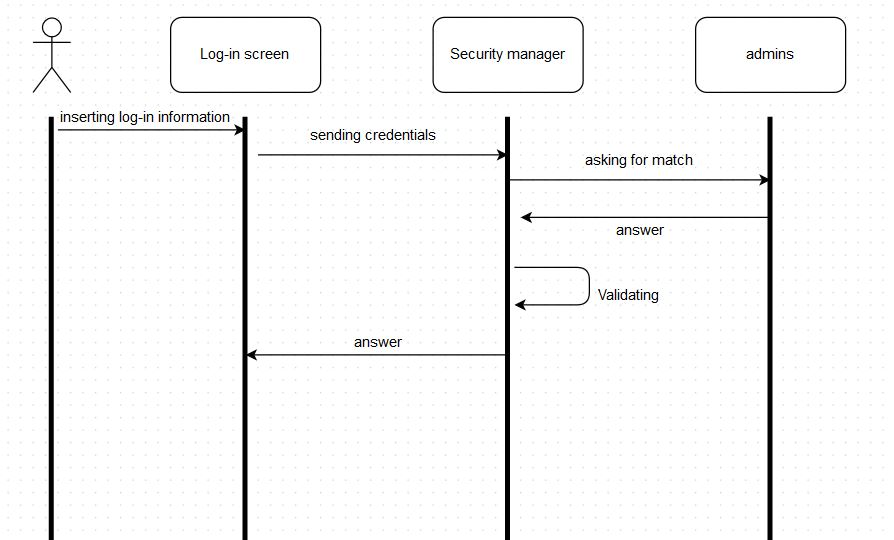
\includegraphics[scale=0.6]{adminLog-in.jpg}
\caption{Sekvens-diagram over use-casen Login}
\end{figure}
Figur 4:
Brugeren indtaster sine informationer på login skærmen.
Informationerne sendes til en sikkerhedsvalideringsfunktion.
Funktionen forespørger om et match i admin-databasen.
Denne sender svar tilbage.
Sikkerhedsvalideringsfunktionen validerer forespørgelsen.
Svaret bliver sendt til login skærmen.
\begin{figure}[H]
\centering
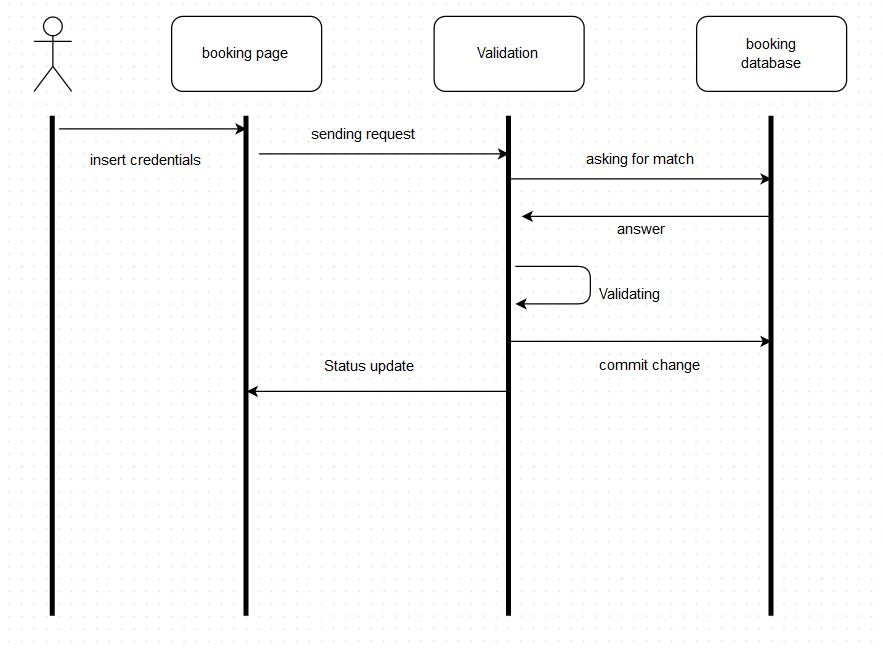
\includegraphics[scale=0.6]{customerLog-in.jpg}
\caption{Sekvens-diagram over use-casen CreateBooking}
\end{figure}
Figur 5:
Brugeren indtaster information på bookingsiden.
Informationen bliver sendt til en valideringsfunktion.
Denne forespørger, om der er konflikter i databasen.
Databasen svarer, og
valideringsfunktionen validerer forespørgelsen.
Status på forespørgsel vises på bookingsiden.
\newpage
\section{Systemdesign sammenfatning}
\textbf{Systemet som det er nu:}
Vi har benyttet Play! frameworket til at lave en meget fin prototype af systemet.
Det er nu muligt at navigere mellem alle de forskellige sider på hjemmesiden. Vi har fået implementeret en billede-slider på siden \textit{Gallery}, som præsenterer billeder af stedet i et diasshow. På siden \textit{Contact} har vi implementeret et google-maps kort, der viser hostelets beliggenhed. Bookingsystemet er også blevet konstrueret, og det er nu muligt at tilføje en booking fra bruger-siden, samt tilføje og slette bookinger fra admin-siden. Bookingerne gemmes i en database.    

\textbf{De væsentligste mangler:}
Vi mangler en funktion, der gør det muligt for administratoren at ændre en booking. Desuden mangler vi stadig at lave et login-system til admin-siden.\\
Vi skal også gøre det muligt for kunden, selv at bestemme hvilke billeder der fremvises samt redigere i teksten på de forskellige sider. Endeligt mangler vi at koble bookingsystemet til et betalingssystem.
\section{Program- og systemtest}
Resultatet af vores testplan er vedlagt som bilag.
\newpage
\section{Brugergrænseflade og interaktonsdesign}
Dette afsnit omhandler brugergrænsefladen og interaktionendesignet, for vores system. 
\subsection{Eksempler på brugergrænseflade}
Følgende billeder viser brugergrænsefladen på hjemmesiden.\\\\
I figur 6 ses vores bookingside hvorfra man kan oprette en booking. 
Det forløbige design er således, at der udover den oblikatoriske menu-bar 
også er fire tekstfelter, en "drop-down" menu og en knap.
Disse felter skal indsamle det data, der bliver til en oprettet booking 
(Indholdet af en booking er ikke færdigt endnu, 
der vil altså være andre/anderledes parametre i slutproduktet). 
\begin{figure}[H]
\centering
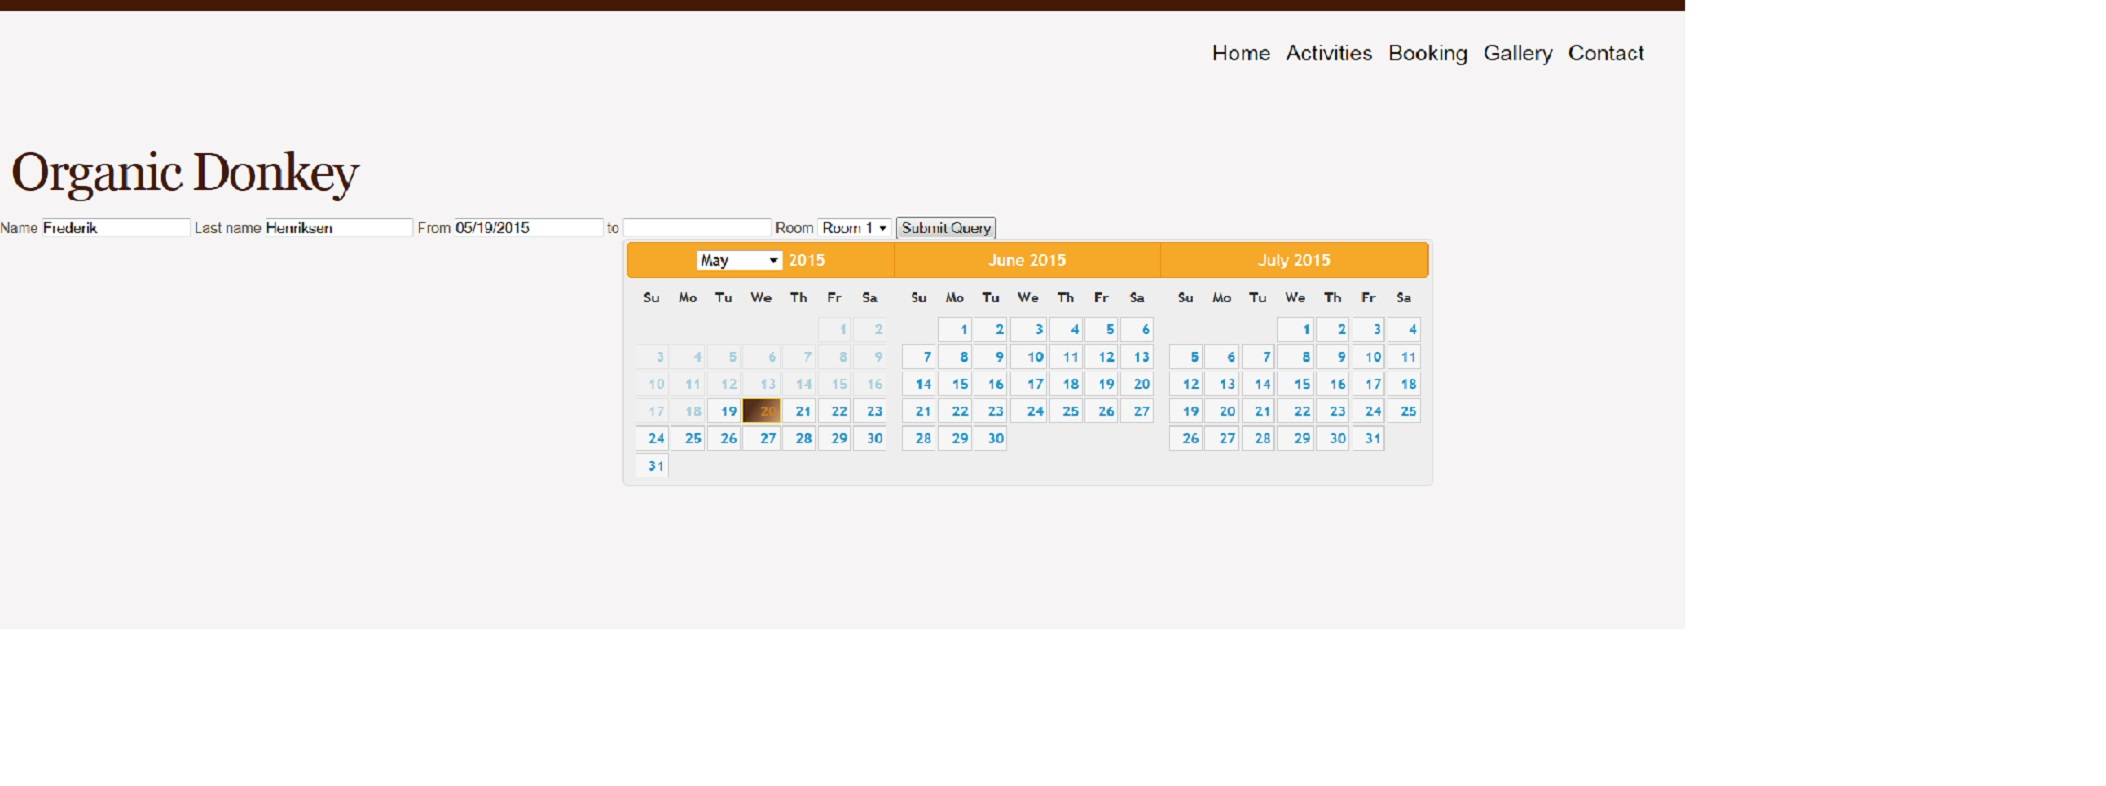
\includegraphics[scale=0.5] {brugergransefladebilled1.jpg}
\caption{Opretter en booking. Her ses en bookning der er ved at blive lavet, hvor brugeren er ved at vælge dato}
\end{figure}
\newpage
I figur 7 ses det layout som går igen på de fleste sider
 med overskrift, menu-bar og tekst.
\begin{figure}[H]
\centering
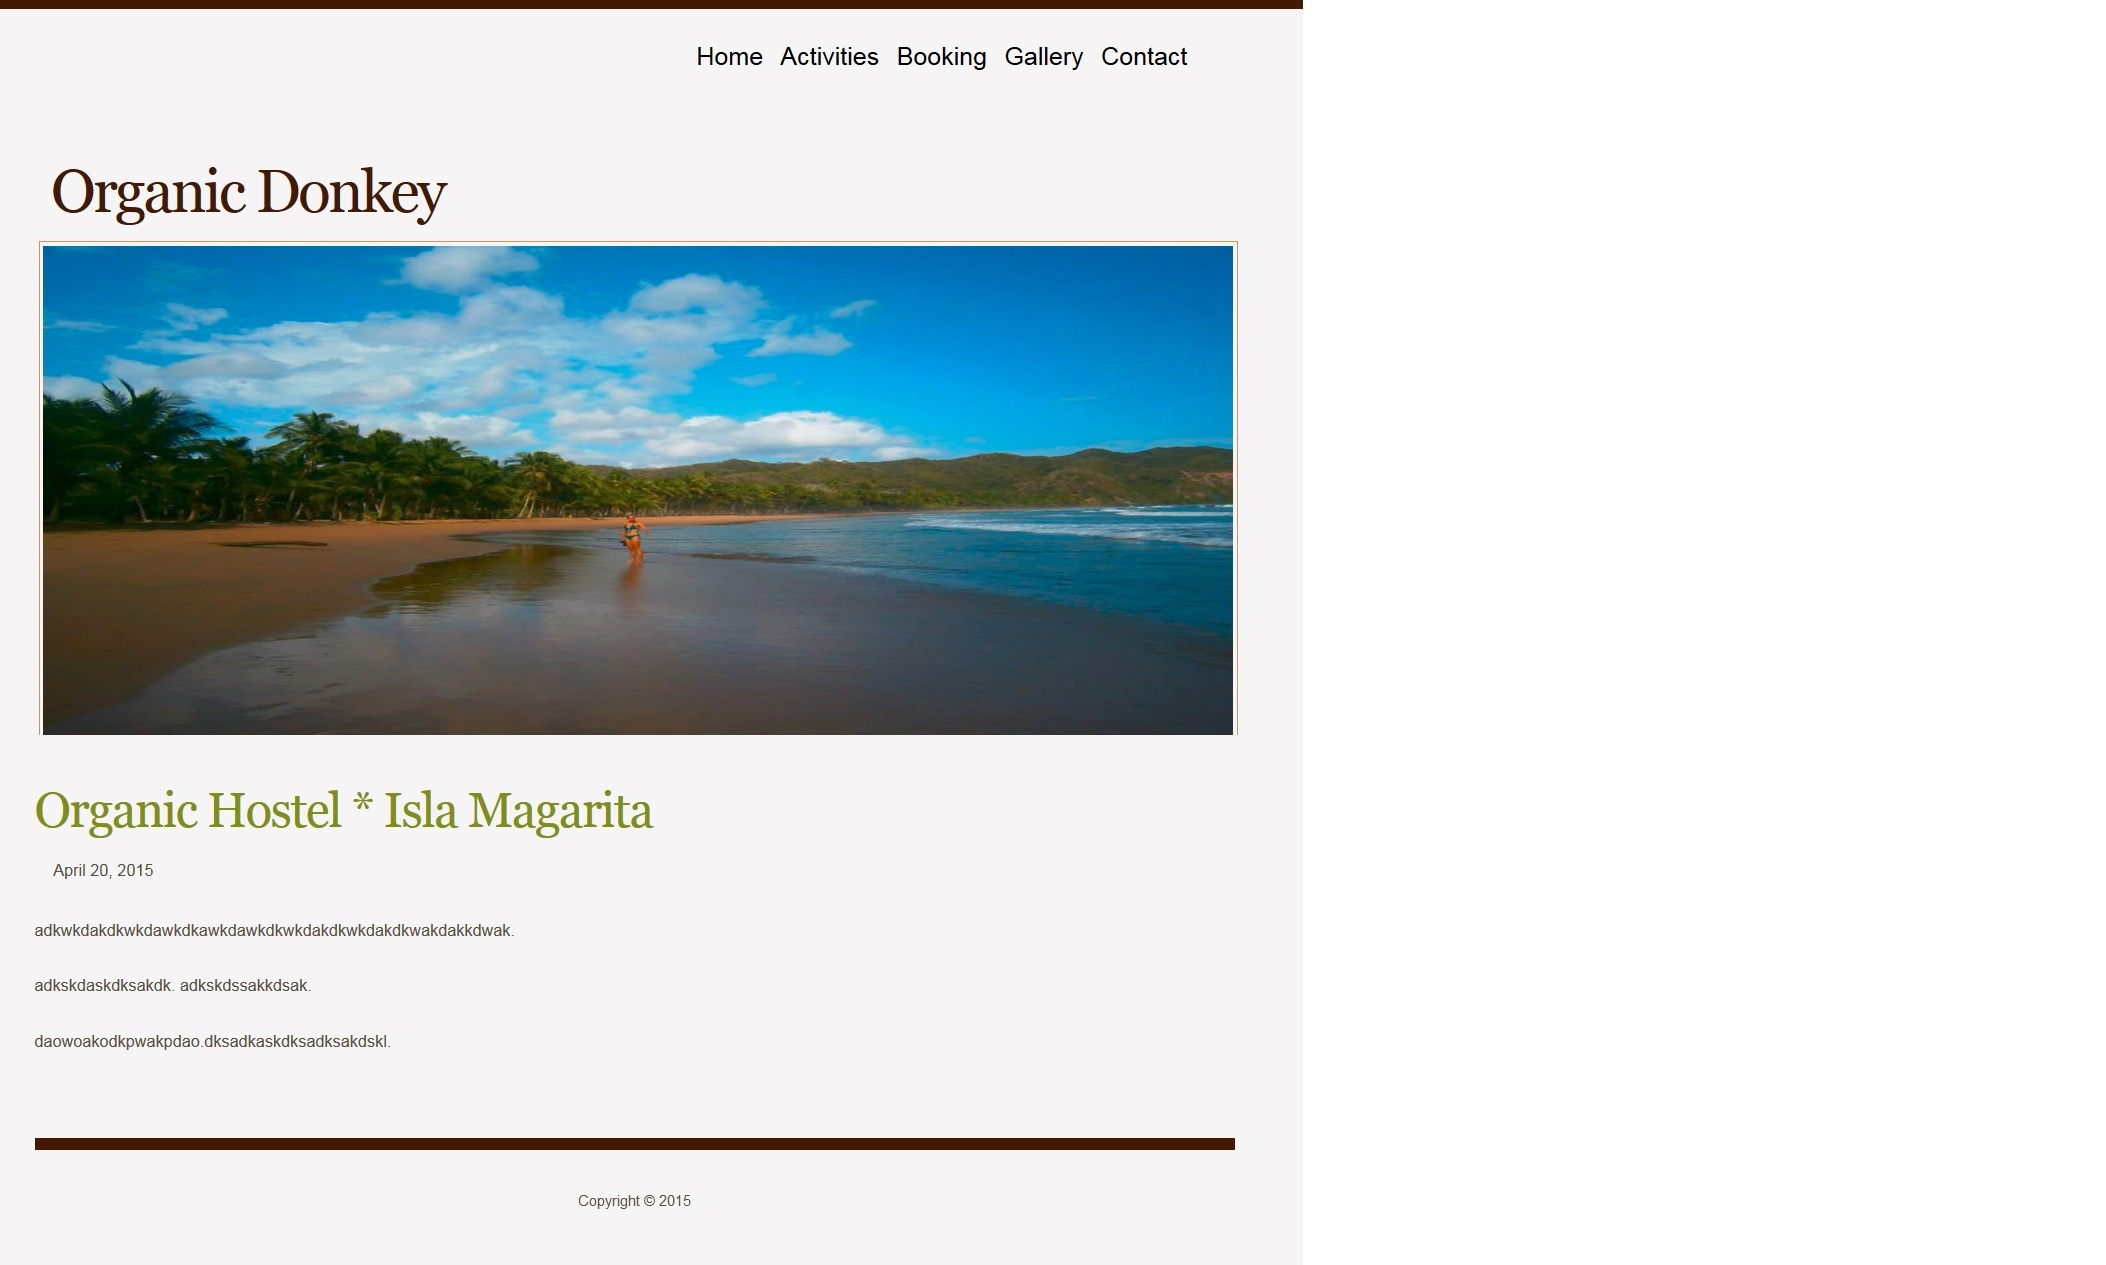
\includegraphics[scale=0.6] {brugergransefladebilled2.jpg}
\caption{Index siden. Her ses vores sides forside} 
\end{figure} 
\newpage
I figur 8 ses den forløbige admin side hvor administrator har overblikket
over bookinger. Administratoren kan søge og slette i bookinger. 
\begin{figure}[H]
\centering
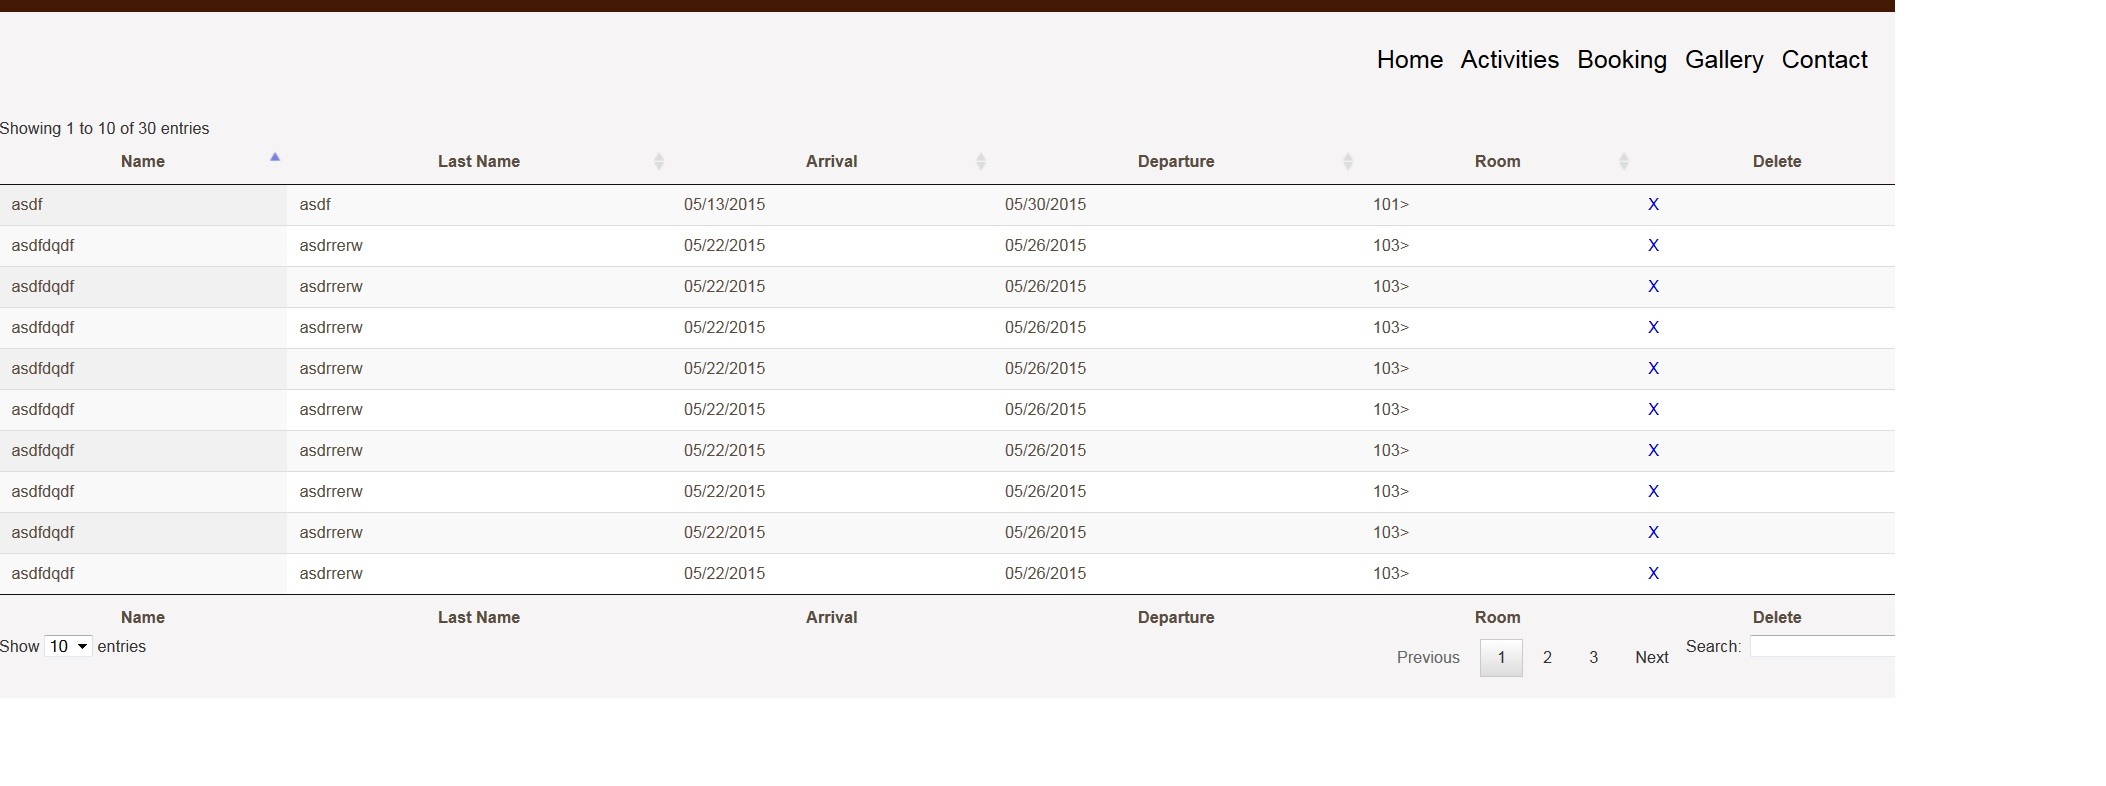
\includegraphics[scale=0.4] {brugergransefladebilled3.jpg}
\caption{Oprettede bookinger. Her ses admin-siden hvor administratoren kan se og redigere bookinger}
\end{figure}

\subsection{Dynamikken i brugerinteraktion}
I figur 9 ses rutediagrammet over, 
hvordan brugere af siden kan bevæge sig imellem de forskellige views. 
Kunden betjener siderne gennem menuen.
Administratoren skal logge ind for at administrere bookingerne.
\begin{figure}[H]
\centering
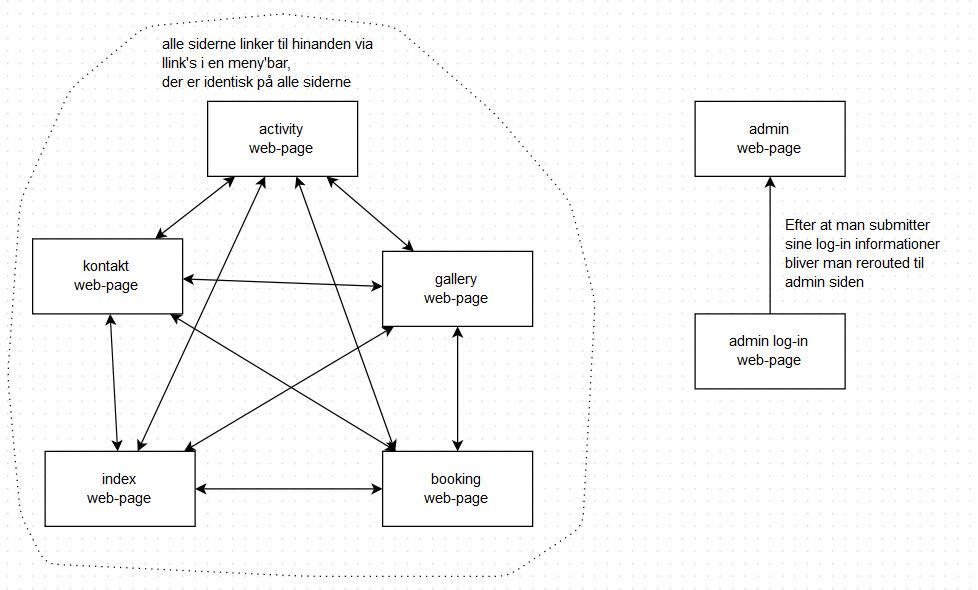
\includegraphics[scale=0.6] {flowchart.jpg}
\caption{Flowchart over siden. Her ses rutediagrammet over siden, som den fungerer på nuværende tidspunkt}
\end{figure}
\newpage
\subsection{Audio-visual præsentation}
Følg linket for at se en audio-visual præsentation af brugergrænsefladen af vores seneste prototype:\\
https://youtu.be/CF55ggqy9M8
\section{Projektsamarbejdet}
Internt i gruppen arbejder vi godt sammen. Cirka halvvejs inde i projektet aftalte vi at sætte mere tid af til projektet. Siden da er vi nået rigtig langt med systemet. 

Vi har indtil videre haft fire møder med kunden. Møderne foregår over Skype, da kunden bor i Venezuela. På trods af at afstanden kan være upraktisk, er kunden fleksibel med dato for møder, da vi blot mødes over Skype.

Under møderne tager vi referat i form af stikord, og dokumenterer de aftalte ændringer i projektaftalen og projektplanen, i rapporten. 
\section{Litteraturreview}
\subsection{Jim Highsmith: Extreme Programming - review}
Extreme Programming er en software udviklings metode, der er karakteriseret ved at være åben for tilpasninger løbende i udviklingsprocessen, som har til hensigt at gøre kvaliteten og reagerer på ændringer i kundes krav. Andre elementer ved extreme programming inkluderer, parprogrammering eller lav en stor kode gennemgang, unit testing af alt koden, og undgå at programmere features før de faktisk skal benyttes og forvent ændringer i kundens krav som tiden går.
\\
\\
Metoden har fire hovedprincipper
\begin{itemize}
	\item Kommunikation
		\begin{itemize}
			\item Brugere og udviklere skal kommunikerer løbende om systemet, så brugeren på en måde kan være med i udviklings processen.
		\end{itemize}
	\item Simpelhed
		\begin{itemize}
			\item Software udvikleren skal kun skrive kode der løser det problem de har her og nu og vil ikke løse problemer der muligvis kan opstå senere.
		\end{itemize}
		\item Feedback
			\begin{itemize}
				\item Der skal laves test, for at udvikleren kan se om det der er lavet virker som antaget.
			\end{itemize}
		\item Mod
			\begin{itemize}
				\item Det kræver mod at lade vær med at bruge de traditionelle udviklings metoder.
			\end{itemize}
\end{itemize}
Extreme programming opererer med tolv punkter, der beskriver måden at arbejde i et extreme programming projekt i praksis.
\begin{itemize}
	\item Planlægning
		\begin{itemize}
			\item Kort 2-3 ugers cyklus, mange udgivelser.
		\end{itemize}
	\item Små udgivelser
		\begin{itemize}
			\item Alle udgivelser skal være så små som mulige, kun indeholde de mest værdifulde krav.
		\end{itemize}
	\item Systemmetafor
		\begin{itemize}
			\item Extreme programming bruger ordet metafor som en måde til at definere det overordnet mål med projektet.
		\end{itemize}
	\item Simpelt design
		\begin{itemize}
			\item Det simple design har to dele, et design for funktionaliteten. To, lave det bedste design der kan give den funktionalitet. 
		\end{itemize}
	\item Hyppige refaktorering
		\begin{itemize}
			\item Designet bliver hyppigt lavet om da kundens krav kan ændre sig.
		\end{itemize}
	\item Test
	\item Parprogrammering
	\item Fælles ejerskab til programkoden
	\item Kontiuerlig integration
	\item Overkommeligt arbejdstempo
	\item Et samlet udviklingshold
	\item Fælles kodestandard
\end{itemize}
I vores projekt har vi lavet lidt af en kombination af extreme programming og den mere traditionelle måde at gribe et system udviklings projekt an. Blandt andet har vi ikke implementeret ting i vores projekt før vi faktisk skulle bruge dem, vi tager en ting af gangen og prøver ikke tænke for langt fremad og kun programmere så tingene kun gør det de skal, uden nogle ekstra features. På den mere traditionelle måde har vi holdt os stramt til vores kunde specifikationer.

\section{Bilag}

\subsection{Bilag 1: Versionsstyring}
Link til vores commit-log på GitHub:\\
https://github.com/fumpen/pksu/commits/master
\subsection{Bilag 2: Changelog for projektrapporten}
Jeppe Schönemann Skov - JSS\\
Frederik Leed Henriksen - FLH\\
Rose Sofie Greve - RSG\\

\begin{table}[h]
\begin{tabular}{lllll}
\cline{1-4}
\multicolumn{1}{|l|}{Initialer} & \multicolumn{1}{l|}{Dato} & \multicolumn{1}{l|}{Afsnit} & \multicolumn{1}{l|}{Ændring} &  \\ \cline{1-4}
\multicolumn{1}{|l|}{JSS, FLH, RSG}     & \multicolumn{1}{l|}{23.04.15}     & \multicolumn{1}{l|}{Alle}       & \multicolumn{1}{l|}{Release edition 1.0}        &  \\ \cline{1-4}
\multicolumn{1}{|l|}{RSG}     & \multicolumn{1}{l|}{07.05.15}     & \multicolumn{1}{l|}{1, 2}       & \multicolumn{1}{l|}{Stavefejl, mere præcis beskrivelse}        &  \\ \cline{1-4}
\multicolumn{1}{|l|}{RSG}     & \multicolumn{1}{l|}{07.05.15}     & \multicolumn{1}{l|}{3.a}       & \multicolumn{1}{l|}{Krav i stikord, mere uddybende}        &  \\ \cline{1-4}
\multicolumn{1}{|l|}{FLH}     & \multicolumn{1}{l|}{07.05.15}     & \multicolumn{1}{l|}{3.b, 3.c, 3.e}       & \multicolumn{1}{l|}{Omskrivning og ændring i model}        &  \\ \cline{1-4}
\multicolumn{1}{|l|}{JSS}     & \multicolumn{1}{l|}{07.05.15}     & \multicolumn{1}{l|}{3.d}       & \multicolumn{1}{l|}{Opdateret klassediagramet}        &  \\ \cline{1-4}
\multicolumn{1}{|l|}{RSG, JSS}     & \multicolumn{1}{l|}{07.05.15}     & \multicolumn{1}{l|}{3.f}       & \multicolumn{1}{l|}{Kommentarer til firgurer}        &  \\ \cline{1-4}
\multicolumn{1}{|l|}{RSG, JSS}     & \multicolumn{1}{l|}{07.05.15}     & \multicolumn{1}{l|}{6, 7}       & \multicolumn{1}{l|}{Ændring i tekst}        &  \\ \cline{1-4}
\multicolumn{1}{|l|}{RSG}     & \multicolumn{1}{l|}{11.05.15}     & \multicolumn{1}{l|}{4, 5, 7}       & \multicolumn{1}{l|}{Ændring i tekst}        &  \\ \cline{1-4}
\multicolumn{1}{|l|}{FLH}     & \multicolumn{1}{l|}{11.05.15}     & \multicolumn{1}{l|}{6}       & \multicolumn{1}{l|}{Flowchart, skærmbilleder, video}        &  \\ \cline{1-4}
\multicolumn{1}{|l|}{RSG}     & \multicolumn{1}{l|}{21.05.15}     & \multicolumn{1}{l|}{3.1 a}       & \multicolumn{1}{l|}{Ændring i tekst}        &  \\ \cline{1-4}
\multicolumn{1}{|l|}{RSG}     & \multicolumn{1}{l|}{27.05.15}     & \multicolumn{1}{l|}{3.1 b}       & \multicolumn{1}{l|}{Nyt diagram}        &  \\ \cline{1-4}
\multicolumn{1}{|l|}{RSG}     & \multicolumn{1}{l|}{27.05.15}     & \multicolumn{1}{l|}{3.1 c}       & \multicolumn{1}{l|}{Ændring af entry og exit conditions}        &  \\ \cline{1-4}
\multicolumn{1}{|l|}{FLH}     & \multicolumn{1}{l|}{27.05.15}     & \multicolumn{1}{l|}{3.1 f}       & \multicolumn{1}{l|}{Beskrivende tekst til diagrammerne}        &  \\ \cline{1-4}
\multicolumn{1}{|l|}{FLH}     & \multicolumn{1}{l|}{27.05.15}     & \multicolumn{1}{l|}{9.3 Timeline}       & \multicolumn{1}{l|}{Beskrivende tekst til diagrammerne}        &  \\ \cline{1-4}
\multicolumn{1}{|l|}{JSS}     & \multicolumn{1}{l|}{02.06.15}     & \multicolumn{1}{l|}{9.4 Testplan}       & \multicolumn{1}{l|}{Beskrivende tekst til diagrammerne}        &  \\ \cline{1-4}
\multicolumn{1}{|l|}{JSS, FLH, RSG}     & \multicolumn{1}{l|}{02.06.15}     & \multicolumn{1}{l|}{Udvidet prototype klar}       & \multicolumn{1}{l|}{Beskrivende tekst til diagrammerne}        &  \\ \cline{1-4}
                           &                           &                             &                              & 
\end{tabular}
\end{table}
\subsection{Bilag 3: Timeline}
-Under første møde d. 19. februar 2015 fik vi lavet en projektaftale med kunden.\\
-Under andet møde d. 10. marts 2015 snakkede vi detaljer ift. bookingsystemet.\\
-Under tredje møde d. 15. april 2015 snakkede vi om valg af betalingssystem, samt om hvilke dele
af projektet kunden helst så os nedprioritere i tilfælde af tidspres.\\
-Den 11 maj 2015 havde vi den første prototype. Denne var i stand til at
oprette bookinger, slette bookinger, sortere bookninger og den havde næste
 alle de sider som der skal være i det endelige produkt.
-Den 2 juni havde vi en udvidet prototype klar.

\subsection{Bilag 4: Test plan}
Vi har ikke til hensigt at tjekke alle typer input eller tjekke sikkerheden af vores kode. 

\paragraph{Systemoversigt}	
Vores program er delt op efter Model-View-Control design mønstret. 

\paragraph{Test og mangler}
Det er primært vores Views der er blevet testet. De eneste tjek, vi har lavet på selve systemet eller databasen, er, om bookingerne bliver lagt over i databasen, når de er blevet submittet, og at de kan blive slettet af administratoren hvis det er ønsket. Samt tjek af login for administratoren. 

\paragraph{Hardware og software krav}
\begin{itemize}
	\item Styresystem der kører OSX, Linux eller Windows
	\item Java
	\item Play Framework
	\item Sqlite
	\item Testet på Chrome og Firefox
\end{itemize}
\paragraph{Prøve plan}
\begin{itemize}
	\item Tilføj booking
	\item Slet booking
	\item Admin login
	\item Admin tilføj / fjern billeder
	\item Admin ændre tekst
\end{itemize}
Vi laver vores test løbende med at de bliver implementeret, så vi har mulighed for at rette systemet til, hvis det skulle påvirke noget af det resterende.

\subsubsection{Test plan specification}
\paragraph{Admin:}
\subparagraph{Login system}
\subparagraph{Test item}
\begin{enumerate}
\item Login med forkert kode
\end{enumerate}
\subparagraph{Output}
\begin{enumerate}
\item Melder en fejl
\end{enumerate}
\paragraph{Alle brugere:}
\subparagraph{Tilføj booking}
\subparagraph{Test item}
\begin{enumerate}
\item Tilføj en booking der starter i fortiden
\item Tilføj en booking der slutter i fortiden
\item Tilføj en booking på et værelse der allerede er fuldt booket
\end{enumerate}
\subparagraph{Output}
\begin{enumerate}
\item Melder en fejl og beder kunden om at ændre tiden
\item Melder en fejl og beder kunden om at ændre tiden
\item Melder en fejl og beder kunden om at vælge et andet værelse
\end{enumerate}
\paragraph{Admin:}
\subparagraph{Slet booking}
\subparagraph{Test item}
\begin{enumerate}
\item Slet en booking
\end{enumerate}
\subparagraph{Output}
\begin{enumerate}
\item Beder admin om acceptere eller cancel ønske om at fjerne bookingen
\end{enumerate}
\paragraph{Admin:}
\subparagraph{Ændre gallery}
\subparagraph{Test item}
\begin{enumerate}
\item Tilføj gyldigt billede
\item Tilføj ugyldigt billede
\item Slet billede
\end{enumerate}
\subparagraph{Input specifikation}
\begin{enumerate}
\item Jpg, png format
\item Forkert format
\end{enumerate}
\subparagraph{Output}
\begin{enumerate}
\item Beder admin accept / cancel
\item Melder fejl og beder admin tjekke om billedet er gyldigt
\item Beder admin accept / cancel
\end{enumerate}
\paragraph{Admin:}
\subparagraph{Ændre tekst}
\subparagraph{Test item}
\begin{enumerate}
\item Tilføj tekst
\item Slet tekst
\end{enumerate}
\subparagraph{Output}
\begin{enumerate}
\item Beder admin accept / cancel
\item Beder admin accept / cancel
\end{enumerate}
\end{document}
